Two types of domino-like rectangular tiles,

\includegraphics[height=1.5ex]{vtrmc-2000-problem7-tile-2-1.eps} and

\includegraphics[height=1.5ex]{vtrmc-2000-problem7-tile-2-2.eps} are available.
The first type may be rotated end-to-end to produce a tile of type

\includegraphics[height=1.5ex]{vtrmc-2000-problem7-tile-1-2.eps}. Let $A(n)$ be
the number of distinct chains of $n$ tiles, placed end-to-end, that may be
constructed if abutting ends are required to have the same number of dots.

\textbf{Example:} $A(2) = 5,$ since the following five chains of length two, and no
others, are allowed.

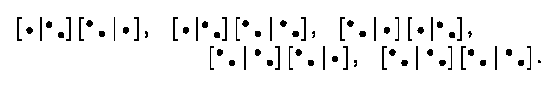
\includegraphics{vtrmc-2000-problem7-tile-example-chain.eps}

\begin{enumerate}[(a)]
\item Find $A(3)$ and $A(4)$.
\item Find, with proof, a three-term recurrence formula for $A(n + 2)$ in terms
      of $A(n + 1)$ and $A(n)$, for $n = 1, 2, \dots$, and use it to find $A(10)$.
\end{enumerate}
